\chapter{Guide}
\label{guide}
In this section I am going to discuss the various pages of the app, 
I am also going to give a brief description of the various components in each page,
and how a user can interact with them.
Most parts of the user interface, such as buttons, text fields, and menu items are meant 
to be obvious and intuitive, so they
do not require any sort of special training for users to learn how they work,
and I will discuss them only briefly here. 
But the user interface of this app also contains a few custom interactions that are specific
to each algorithm. The purpose of this section is to outline those interactions.
Note that some of the details (and images) in this section are subject to minor changes 
in the live version of the app.
I recommend reading this section with colors (as opposed to black an white), 
because some of the figures become hard to understand in black and white.
%%%%%%%%%%%%%%%%%%%%%%%%%%%%%%%%%%%%%%%%%%%%%%%%%%%%%%%%%%%%%%%%%%%%%%%%%%%%%%%%%%%
\section{Home Page}
\begin{figure}[H]
  \caption{Home Page}
  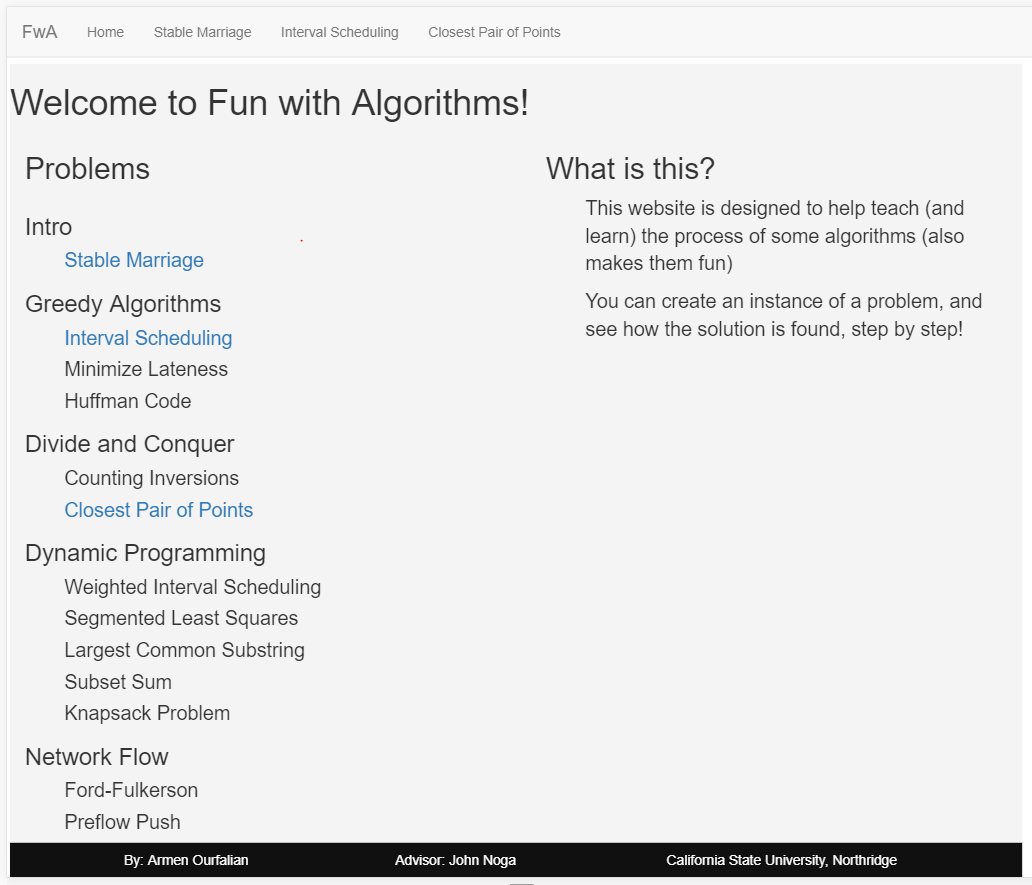
\includegraphics[
  height = 3.5in
  ]{images/home-screen.png}
  \label{fig-home-screen}
  \centering
\end{figure}
\hspace{-0.3in}
The app can be found at \underline{http://funwithalgorithms.herokuapp.com/}
The home page is the first page that you will see
\textit{(Figure \ref{fig-home-screen})}. 
It contains a list of topics, some in black others in blue.
The topics are
organized by Algorithm type (Greedy, Divide and Conquer, etc.) 
These are a subset of algorithms covered in an intermediate Algorithms class. 
The topics in black are a potential list of future topics to be covered.
The topics that have already been created for the app are in blue,
and they are links that lead to their corresponding page. 
There is also a link to each topic in the navigation bar. 
To return to the home screen, you can click on the far-left link 
in the navigation bar (FwA).
%%%%%%%%%%%%%%%%%%%%%%%%%%%%%%%%%%%%%%%%%%%%%%%%%%%%%%%%%%%%%%%%%%%%%%%%%%%%%%%%%%%
\section{Reusable Components}
\hspace{-0.3in}
As mentioned in \textbf{Chapter \ref{tools-and-technologies} Tools and Technologies}, 
a key feature of Vue is reusable components. So a number of components in this app 
are shared across multiple algorithms.
Reusing components across various pages gives the website 
a more consistent feel overall and 
reduces the amount of training required to use the app. 
I packed the majority of the reusable functionalities into the secondary 
navigation bar (navbar) \textit{(Figure \ref{fig-second-nav})} 
to ensure they would be easy to find no matter what page the 
user found themselves on. 
\subsection{The Second Navbar}
\begin{figure}[H]
  \caption{Second Navbar}
  
\includegraphics[
  width = \textwidth
  ]{images/reusable-components/second-nav.png}
  \label{fig-second-nav}
  \centering
\end{figure}
The second navbar appears on every algorithm page, just below the regular navbar.
It has a black background, which contrasts with the first navbar. 
While the first navbar allows navigation across the various pages of the app, 
the second navbar serves more as a menu bar with dropdown menus and other tools.
The key features of the second navbar are discussed in the next few subsections. 
\subsection{File Menu}
\begin{figure}[H]
  \caption{File Menu}
  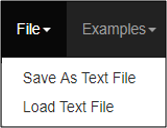
\includegraphics[
  ]{images/reusable-components/file-menu.png}
  \label{fig-file-menu}
  \centering
\end{figure}
\hspace{-0.3in}
A \textbf{File Menu} \textit{(Figure \ref{fig-file-menu})} 
with the options \textbf{Save as Text File} and \textbf{Load Text File}. 
These features should be familiar to the modern user. 
Although the interface to save or load an instance is exactly the same For each problem,
the save and load functionalities are customized for each problem. 
This is because each problem requires a different format for its input data.
\newline\newline
For example: \textsc{Stable Marriage} requires an input of exactly two $n\times n$
lists of numbers, where the numbers 
must be in the range $[0, n-1]$ or $[1, n]$, 
whereas the \textsc{Interval Scheduling} 
requires an input of up to $200$ rows, each containing two numbers $(startTime, finishTime)$.
Despite these differences, the interface for saving or loading instances 
is exactly the same for all problems within the entire project. 
\subsection{Saving and Loading}
\begin{figure}[H]
  \caption{Stable Marriage Save and Load interfaces}
  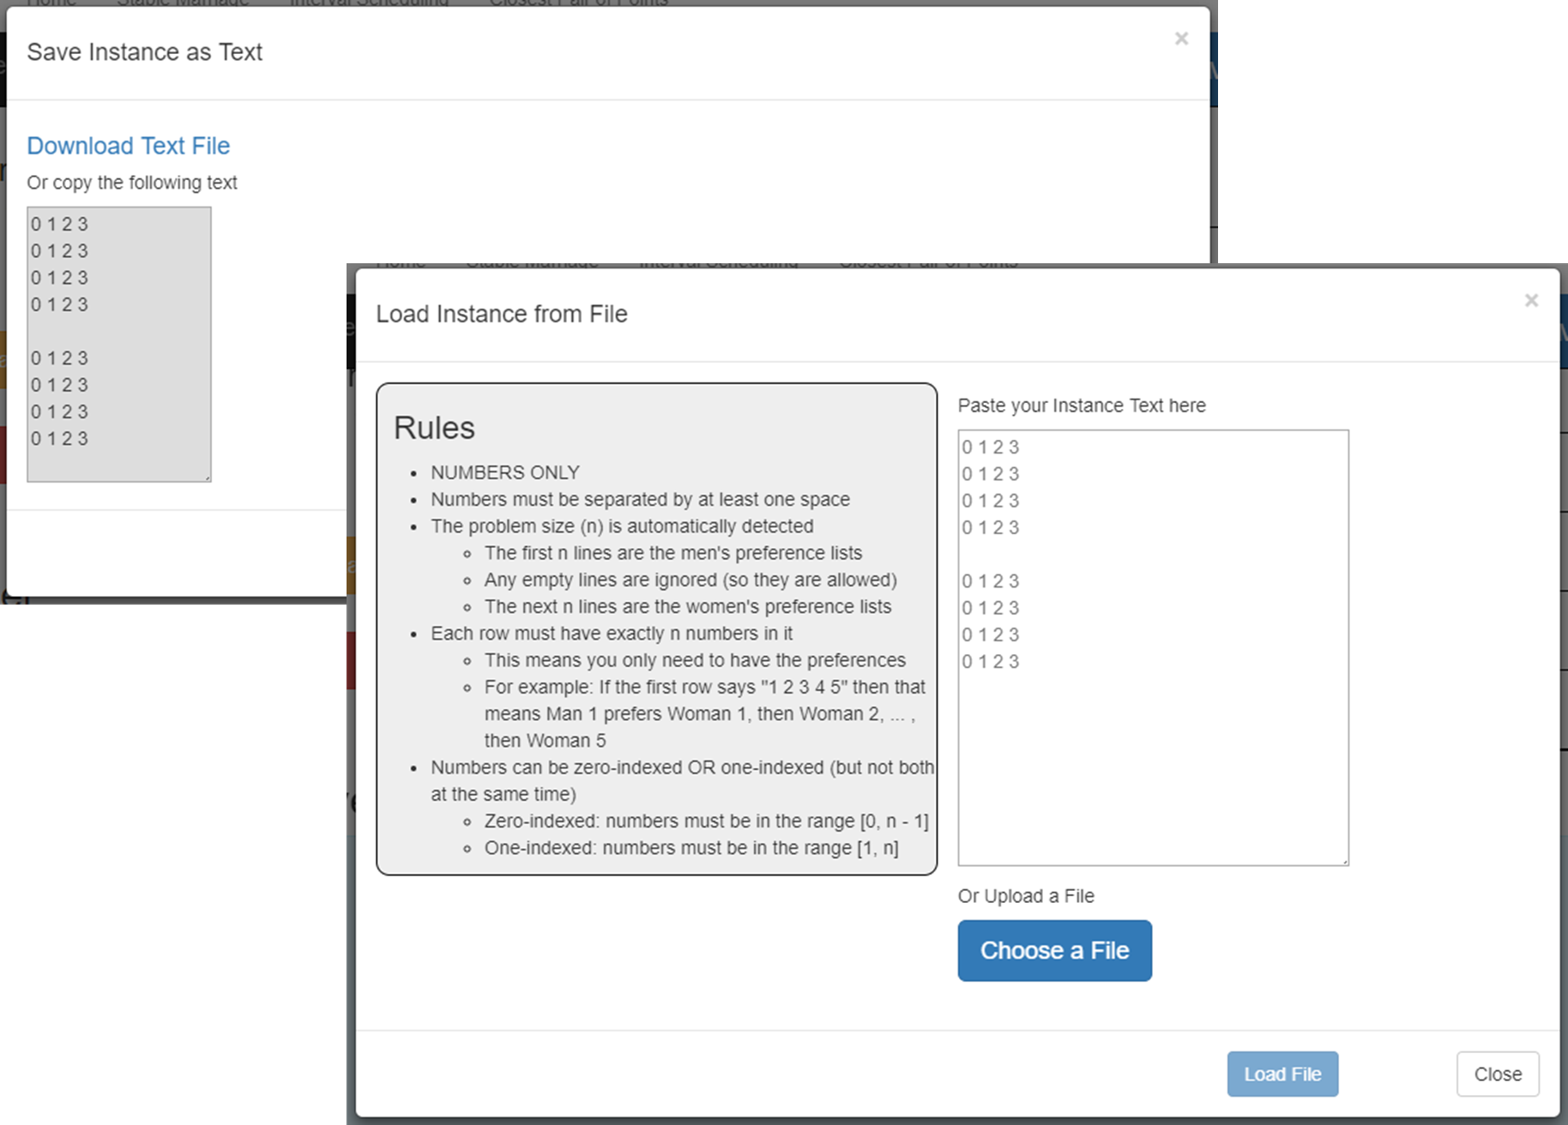
\includegraphics[
    width=\linewidth
  ]{images/reusable-components/save-load.png}
  \label{fig-save-load}
  \centering
\end{figure}
\hspace{-0.3in}
\textit{Figure \ref{fig-save-load}} shows both the Save and Load interfaces 
for Stable Marriage. 
The Save interface is used when a user has made an instance of a problem 
with the app, and wants to save it as a text file on their computer. 
The Load interface is used when a user wants to load an instance from their 
computer onto the app 
(instead of manually creating the instance by interacting with the app). 
\newline\newline
The Save interface shows the text that represents the instance. 
A user can copy this text into a text file manually, or they can click 
the link titled ``Download Text File'' to download a text file directly.
The text itself is meant to be a simple and straightforward representation 
of the instance.
\newline\newline
The Load interface shows a set of rules that are unique to each problem. 
These rules are meant to guide the user on how to create files
that will be accepted by the app.
There is a large text box where the user can paste (or even manually type) 
the instance. 
The placeholder text
(the text that is in a lighter color and usually gives 
hints about what kind of information should be typed into the text box)
of the text box is the same text that the Save interface shows,
this is another hint that is given to the user about
what the text file should look like. 
There is also a button labelled ``Choose a File'' that allows the user
to upload a text file directly. 
\newline\newline
\begin{figure}[H]
  \caption{Stable Marriage Error Message}
  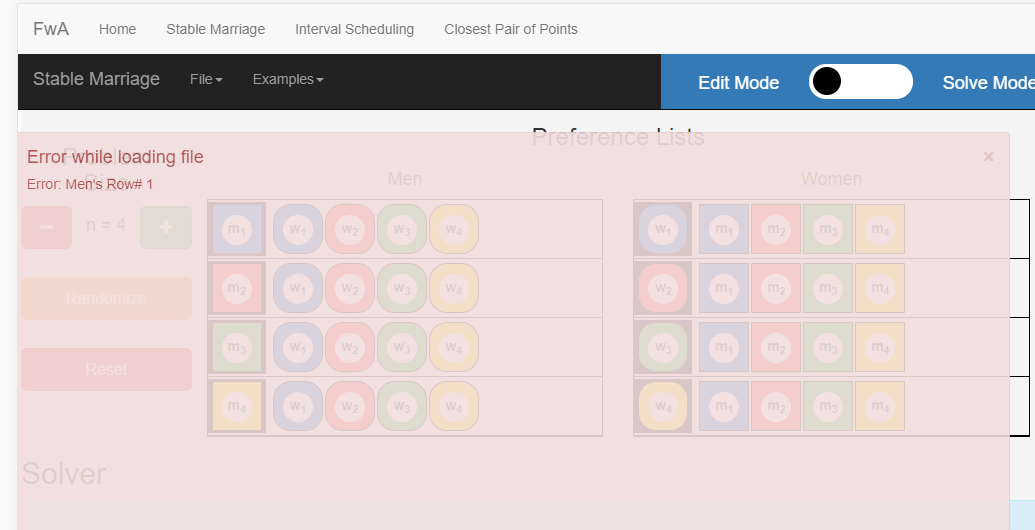
\includegraphics[
  height=2.5in
  ]{images/reusable-components/error-message.png}
  \label{fig-error-message}
  \centering
\end{figure}
Upon clicking the button labelled ``Load File'' If there are any problems with the file, 
the app will display a message in red specifying which line 
contained the error, as seen in \textit{Figure \ref{fig-error-message}}. 
If there are errors in the file, the load may or may not fail completely, 
depending on the algorithm:
Both Stable Marriage and Interval Scheduling only load a file if there are no errors, 
whereas Closest Pair of Points will still load the file, but ignores any lines that had 
errors in them. 

%
\subsection{Examples Menu}
\begin{figure}[H]
  \caption{Examples Menu for Stable Marriage}
  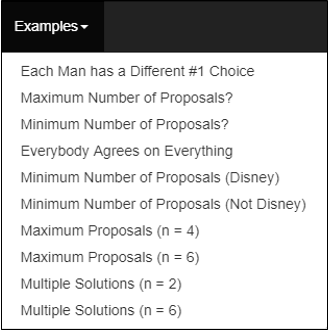
\includegraphics[
  ]{images/reusable-components/example-menu.png}
  \label{fig-example-menu}
  \centering
\end{figure}
\hspace{-0.3in}
Next to the \textbf{File Menu} is an \textbf{Examples Menu} 
\textit{(Figure \ref{fig-example-menu})} 
that contains a list of 
premade instances for each problem. 
These instances are interesting cases that are often brought up
in lecture. 
When a user selects one of the items from this menu, 
that instance is automatically loaded into the current page. 
\subsection{Edit Mode and Solve Mode}
\begin{figure}[h]
  \caption{Edit Mode}
  \label{fig-edit-mode}
  
\includegraphics[]{images/reusable-components/edit-mode.png}
  \centering
  \caption{Solve Mode}
  \label{fig-solve-mode}
  
\includegraphics[]{images/reusable-components/solve-mode.png}
  \centering
\end{figure}
On the far-right side of the second navbar is a switch 
\textit{(Figures \ref{fig-edit-mode} and \ref{fig-solve-mode})} 
that goes between \textbf{Edit Mode} and \textbf{Solve Mode}. 
Edit Mode will display the \textsc{Instance Maker},
whereas Solve Mode will display the \textsc{Solver}. 
In both modes, the \textsc{Display} will also be visible. 
\newline\newline
The functionality of this switch  is the same across all algorithms:
the problem instance can only be changed (\textbf{edited}) when the page is on Edit Mode, 
and algorithm can only be performed (\textbf{solved}) while in Solve Mode. 
The reason for this is because giving the user the ability to change the 
problem instance mid-way through the algorithm would cause unexpected problems
such as infinite loops or divide-by-zero errors in the worst case, and be 
confusing in the best case. 
For this reason, whenever the user switches from Solve Mode into Edit Mode, 
the \textsc{Solver} is completely reset to its initial state, and any progress
made in the algorithm is lost.
\subsection{Automator}
\begin{figure}[H]
  \caption{Automator Component}
  
\includegraphics[width=\linewidth]
  {images/reusable-components/automator.png}
  \label{fig-automator}
  \centering
\end{figure}
Included in some pages is an \textbf{Automator} component. 
\textit{Figure \ref{fig-automator}} shows what this component looks like. 
The \textbf{Automator} will run the algorithm automatically at set time intervals. 
The user can increase or decrease the speed of the Automator within some 
preset limiits. They can also pause the Automator as it is running if they wish
to continue manually from any point. The Automator will be disabled
if the page is in \textbf{Edit Mode} or if the algorithm has already completed.
%%%%%%%%%%%%%%%%%%%%%%%%%%%%%%%%%%%%%%%%%%%%%%%%%%%%%%%%%%%%%%%%%%%%%%%%%%%%%%%%%%%
\section{Stable Marriage}
\begin{figure}[H]
  \caption{Stable Marriage in Edit Mode}
  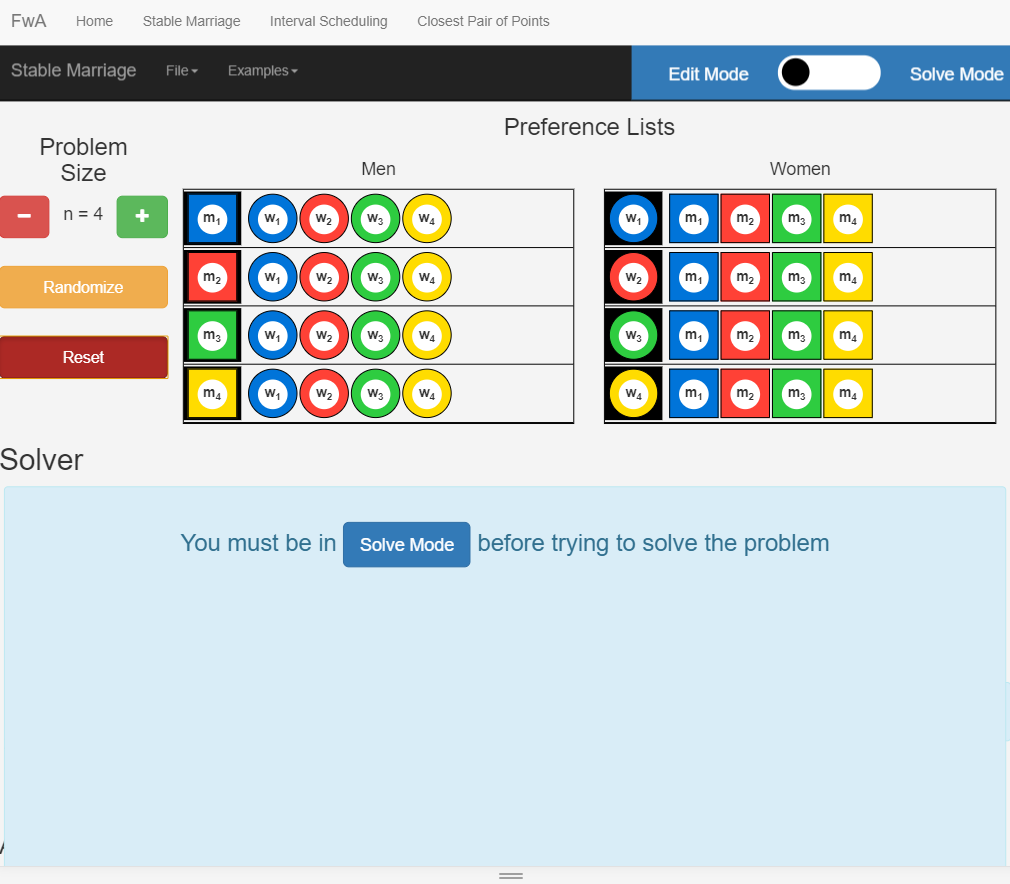
\includegraphics[height=3.5in]
  {images/stable-marriage/stable-marriage-edit.png}
  \label{fig-stable-marriage-edit}
  \centering
\end{figure}
\hspace{-0.3in}
Upon first visiting the Stable Marriage page, 
the user sees a page similar to \textit{Figure \ref{fig-stable-marriage-edit}}.
By default, the page is loaded in \textbf{Edit Mode}, 
with a default instance of size $n=4$. 
\newline\newline
In the center of the page are the two preference lists, each with 4 rows 
(the number of rows is always equal to the Problem Size). 
Each row has five (Problem Size $+1$) 
colorful boxes (squares and circles are both referred to as boxes)
\newline\newline
The first box in each row has a thick border, 
and represents a person (a man or a woman), 
and the rest of the boxes represent 
that person's rankings of the members of the opposite sex.
The further left a person is, the higher they are ranked. 
\newline\newline
\begin{figure}[H]
  \caption{Example Preference Row}
  
\includegraphics[]
  {images/stable-marriage/preference-row.png}
  \label{fig-preference-row}
  \centering
\end{figure}
As an example: in \textit{Figure \ref{fig-preference-row}} 
we can see that $m_2$ ranks $w_4$ as his most preferred choice, 
then $w_1$, then $w_2$, 
and $w_3$ is his least preferred choice.
\newline\newline
The colors correspond to numbers ($1$ is blue, $2$ is red, etc.). 
The purpose of the colors is to create an easier way for students to 
differentiate the various people. 
Note that the fact that the colors are the same for men and women holds no significance
(ie there is no inherent relationship between $m_1$ and $w_1$,
they just both happen to be blue).
The boxes for men are squares and the boxes for women are circles. 
This is to allow students to easily differentiate between each gender. 
\subsection{Instance Maker}
\hspace{-0.3in}
On the left-hand side of the page are four buttons:
\begin{itemize}
  \item\textbf{ $-$ and $+$:} These buttons decrease or increase the problem size, respectively
  \item \textbf{Randomize:} This button will shuffle the preference lists to create a 
  random instance, without changing the problem size
  \item \textbf{Reset:} This button will reset the preference lists to their default 
  position, which is in increasing numerical order
\end{itemize}
Aside from the buttons, the main user interaction with the \textsc{Instance Maker} 
happens directly on the preference lists. 
To edit the preference lists, the user has to reorder the preferences of each person.
This can be done by clicking on any box inside of a preference row 
(except the box on the far-left with the thick border) 
and dragging that box horizontally left and right. 
This will swap that box with its neighbor.
\newline\newline
On a touchscreen device (such as an iPad), this dragging function does not work. 
Instead the user must touch on one box 
(the box will be highlighted in dark grey)
and then touch another box in the same row to swap them.
\newline\newline
In both cases, when the boxes are swapped, they will both rotate $360^o$ in place 
to indicate that they have been changed.
\subsection{Solver}
\begin{figure}[H]
  \caption{Stable Marriage in Solve Mode}
  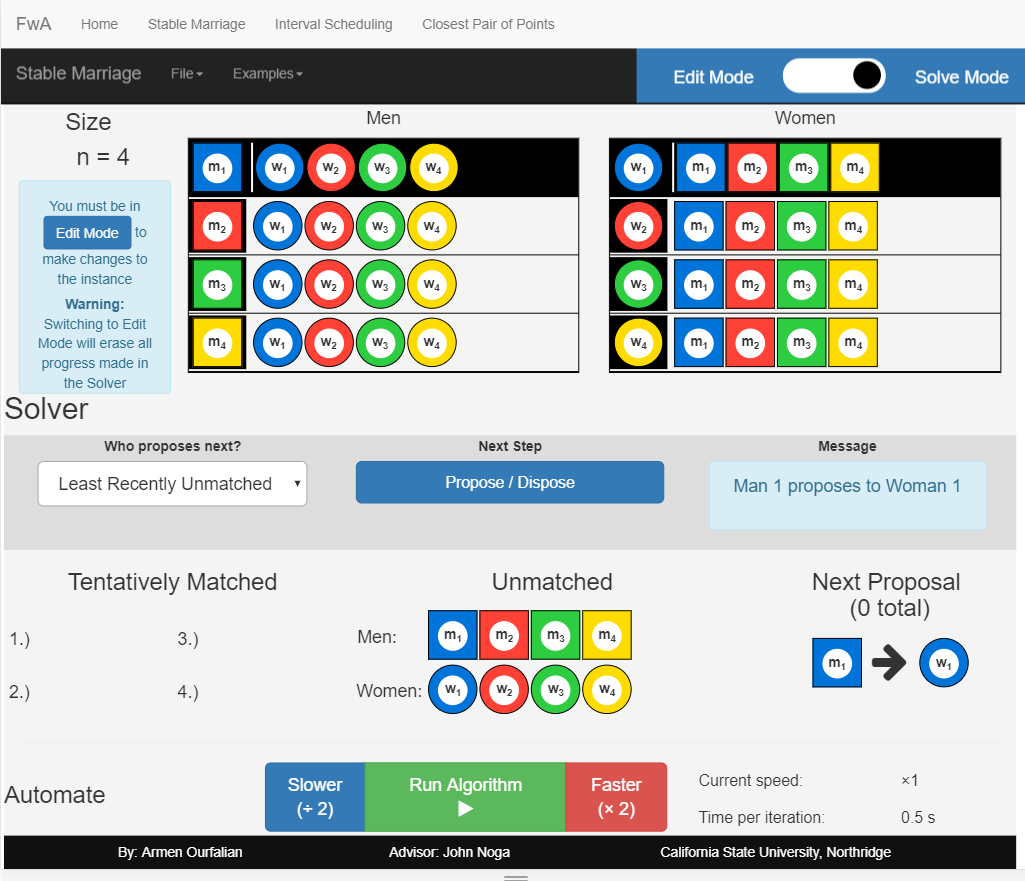
\includegraphics[height=3.5in]
  {images/stable-marriage/stable-marriage-solve.png}
  \label{fig-stable-marriage-solve}
  \centering
\end{figure}
\hspace{-0.3in}
When the page is changed to \textbf{Solve Mode}, the user will see a page similar to 
\textit{Figure \ref{fig-stable-marriage-solve}}. 
In this mode, the buttons of the \textsc{Instance Maker} have been removed, 
but a new set of controls has been made available just below the preference lists:
\begin{itemize}
  \item \textbf{Who Proposes Next:} This is a dropdown menu to determine which 
    man is proposes next. 
    The available options are: 
  \begin{itemize}
    \item \textbf{Least Recently Unmatched:} The man that has gone longest without 
      proposing is the next one to propose. 
      At the beginning when no men have proposed yet, 
      the men propose in increasing order of their number 
    ($m_1$ goes first, then $m_2$, and so on).
    \item \textbf{Most Recently Unmatched:} The opposite of the previous option, 
      the man who has most recently proposed goes next. At the beginning, 
      when no men have proposed yet, the men propose in decreasing order 
      of their number ($m_4$ goes first, then $m_3$ and so on)
    \item \textbf{Choose By Clicking:} When this option is selected, 
      the user decides which man proposes next by clicking on the man's box
      in the Unmatched component.
      The first click makes the man propose, and the second click 
      makes the woman respond. 
      After the second click, the user may click on another man
      (or they may click on the same man again). 
      \subitem Note that if this option is selected, the \textbf{Automator} will be disabled.
    \item \textbf{Random:} In this case, the man who proposes next will be chosen 
      randomly.
  \end{itemize}
  \item \textbf{Next Step:} This button is clicked to perform the next step of 
  the algorithm
  \item \textbf{Message:} The message is a type of feedback that either gives
  instructions to the user 
  (such as ``Click the blue button to perform the next step of the algorithm'')
  or describes which step of the algorithm is being perform 
  (such as ``Man 1 proposes to Woman 1'');
\end{itemize}
Below the controls are three components that
provide useful information as the algorithm is being performed. 
\newline\newline
\begin{figure}[H]
  \caption{Unmatched Component}
  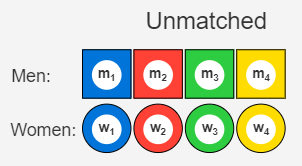
\includegraphics[height=1.25in]
  {images/stable-marriage/unmatched.png}
  \label{fig-unmatched}
  \centering
\end{figure}
In the middle is the list of people who are currently \textbf{Unmatched}. 
This list is useful for discussing which man should propose next, 
and if a woman is unmatched, then she won't reject a proposal from any man. 
Also, if the ``Choose By Clicking'' option is selected
from the \textbf{Who Proposes Next}, then the 
user must click on the men's boxes in the \textbf{Unmatched} component. 
\newline\newline
\begin{figure}[H]
  \caption{Next Proposal Component}
  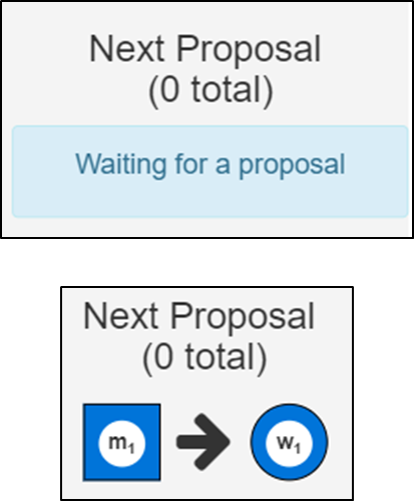
\includegraphics[height=2in]
  {images/stable-marriage/next-proposal.png}
  \label{fig-next-proposal}
  \centering
\end{figure}
To the right is the \textbf{Next Proposal} component, 
which is a graphical representation of a proposal. 
\textit{Figure \ref{fig-next-proposal}} shows some examples 
of the \textbf{Next Proposal} component
\begin{figure}[H]
  \caption{Tentatively Matched Component}
  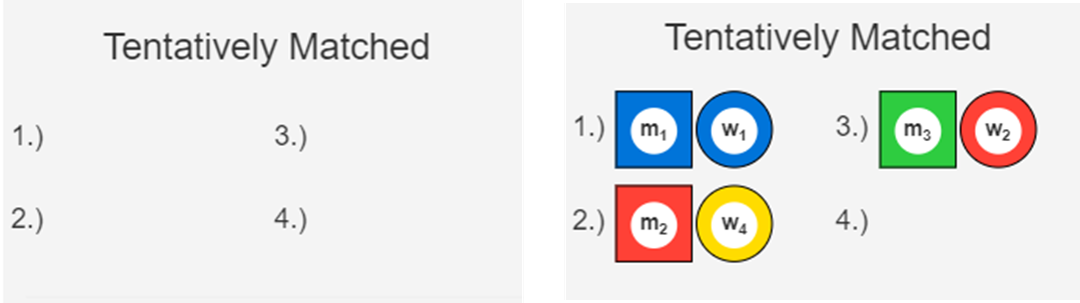
\includegraphics[height=1.25in]
  {images/stable-marriage/tentative.png}
  \label{fig-tentative}
  \centering
\end{figure}
\textit{Figure \ref{fig-tentative}} shows some examples of the 
\textbf{Tentatively Matched} component. 
This component is the complement of the \textbf{Unmatched component} in that
it only shows the people who are currently matched. 
\newline\newline
Although the three components described in this section convey a lot of information,
the user needs to constantly look at the preference lists to determine what 
the algorithm will do next. 1
Since it can be hard to focus on multiple sources of information back and forth, 
the preference lists also communicate much of the same information as these 
sections (albeit more symbolically)
\begin{figure}[H]
  \caption{What the Preference Lists look like in the middle of the Algorithm being performed}
  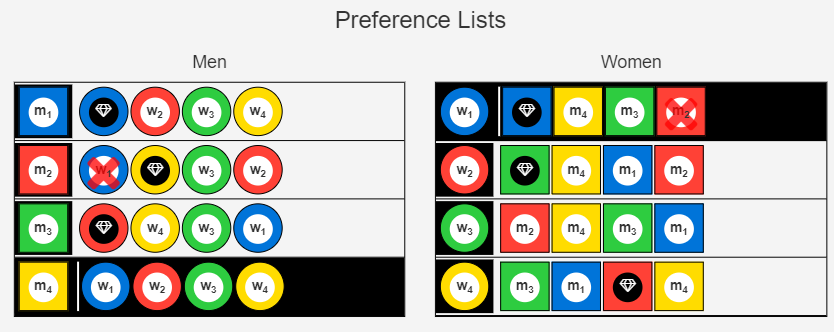
\includegraphics[width=\linewidth]
  {images/stable-marriage/sm-algorithm-running.png}
  \label{fig-sm-algorithm-running}
  \centering
\end{figure}
\textit{Figure \ref{fig-sm-algorithm-running}} is an example of what the
preference lists may look like in the middle of the algorithm.
If a person is part of a tentatively matched couple, their partner's number
is replaced with a white diamond 
(in this case $m_1$ and $w_1$ are tentatively matched, 
$m_2$ and $w_4$ are matched, and $m_3$ and $w_2$ are matched).
If a man has been rejected by a woman, 
that woman's box is crossed out with a red X. 
And if a man is proposing to a woman, their preference rows are highlighted in black. 
%%%%%%%%%%%%%%%%%%%%%%%%%%%%%%%%%%%%%%%%%%%%%%%%%%%%%%%%%%%%%%%%%%%%%%%%%%%%%%%%%%%
\section{Interval Scheduling}
\begin{figure}[H]
	\caption{Interval Scheduling in Edit Mode}
	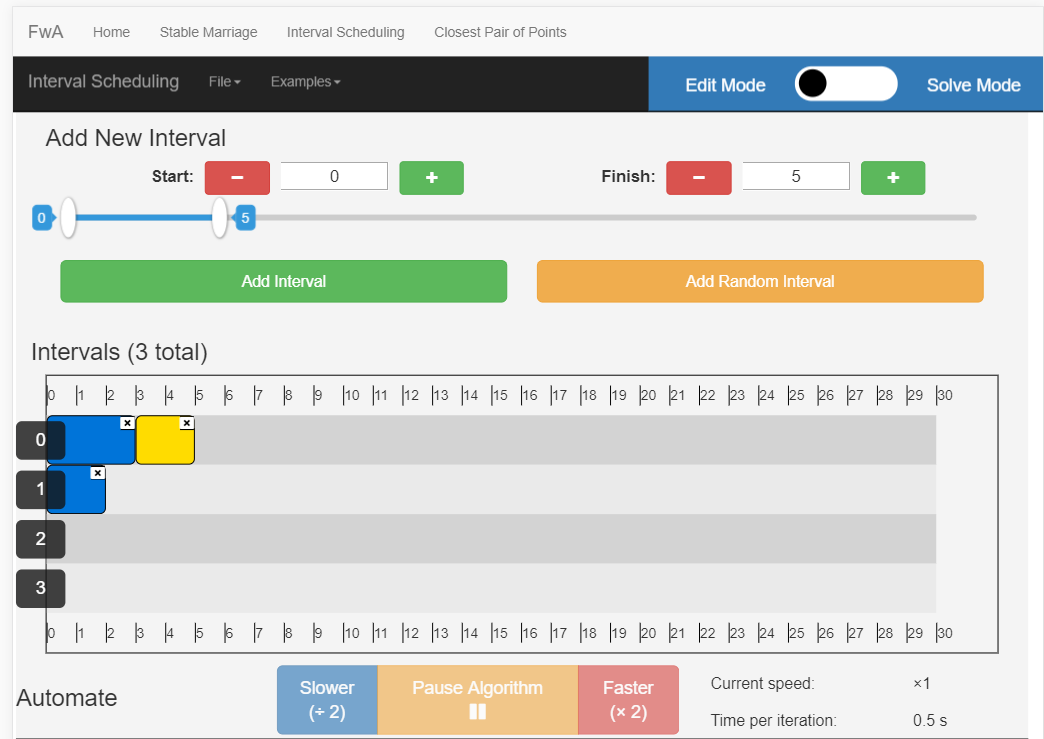
\includegraphics[height=2.5in]
	{images/interval-scheduling/interval-scheduling-edit.png}
	\label{fig-interval-scheduling-edit}
	\centering
\end{figure}
\textit{Figure \ref{fig-interval-scheduling-edit}} shows the Interval Scheduling page
upon first visiting it. 
The top portion of the page represents the \textsc{Instance Maker} and the bottom 
portion represents the \textsc{Display}. 
\subsection{Instance Maker}
\hspace{-0.3in}
The \textsc{Instance Maker} for Interval Scheduling consists of an interface to 
add and delete intervals:
\newline\newline
To delete an interval, the user must click on the small X in the top-right corner 
of the interval in the \textsc{Display}. 
\newline\newline
To add an interval $(startTime, finishTime)$, 
the user can use the $-$ and $+$ buttons, the dual sliders, or even type into the 
text boxes for \textbf{Start} and \textbf{Finish}. All three of these methods
are equivalent, and the user may even mix-and-match between the three methods.
Also, the ``Add Random Interval'' button will add a new interval
with random start and finish times. 
\newline\newline
When the user adds an interval, it gets added to the least-occupied row in the display,
as long as it doesn't overlap with any other intervals already in that row. 
If no such rows exist, then a new row is created and the interval is added to that row.
\subsection{Solver}
\begin{figure}[H]
	\caption{Interval Scheduling in Solve Mode}
	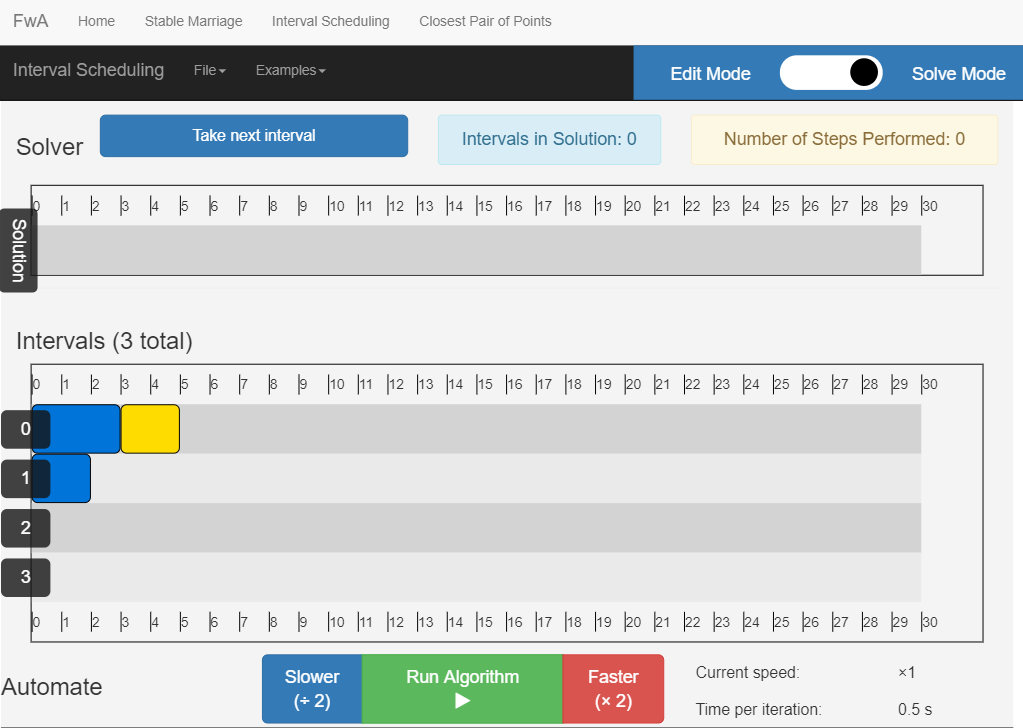
\includegraphics[height=2.5in]
	{images/interval-scheduling/interval-scheduling-solve.png}
	\label{fig-interval-scheduling-solve}
	\centering
\end{figure}
 Switching the page to \textbf{Solve Mode} will
 remove the controls to add and delete intervals, and bring out 
 a new set of controls (which consist of a single button). 
 The blue button alternates between saying ``Take Next Interval'' and 
 ``Remove any intervals that overlap''. The yellow counter on the far right 
 will increase by 1 each time the blue button is clicked. 
 In the middle, the blue counter keeps track of how many intervals 
 are in the solution set. This is the number that an instructor needs to point to
 in front of a confused class and explain that it's the number of intervals that 
 is important, and not some other property of the intervals in the solution set. 
 The row labeled ``Solution'' shows which intervals have been added to the solution. 
 \newline\newline
 As the algorithms is being performed, the interval with the earliest finish 
 time gets added to the Solution row, and any intervals that overlap with it are
 marked with a red X, as seen in \textit{Figure \ref{fig-interval-scheduling-algorithm-runtime}}
 	\begin{figure}[H]
 		\caption{Interval Scheduling Algorithm}
 		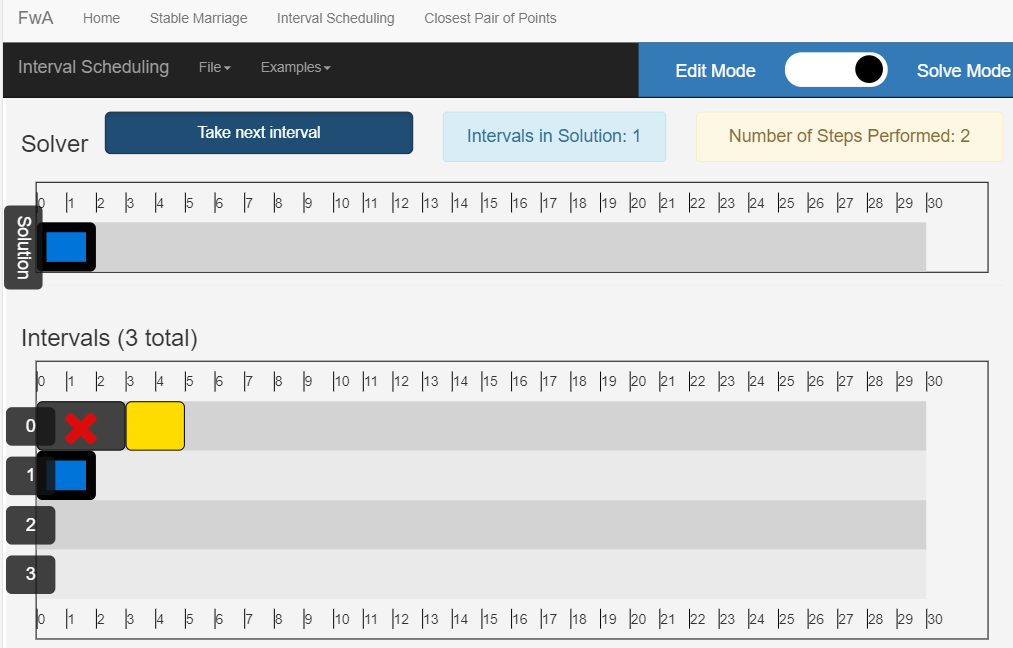
\includegraphics[width=\linewidth]
 		{images/interval-scheduling/interval-scheduling-algorithm-runtime.png}
 		\label{fig-interval-scheduling-algorithm-runtime}
 		\centering
 	\end{figure}
%%%%%%%%%%%%%%%%%%%%%%%%%%%%%%%%%%%%%%%%%%%%%%%%%%%%%%%%%%%%%%%%%%%%%%%%%%%%%%%%%%%
\section{Closest Pair of Points}
\begin{figure}[H]
	\caption{Closest Pair of Points in Edit Mode}
	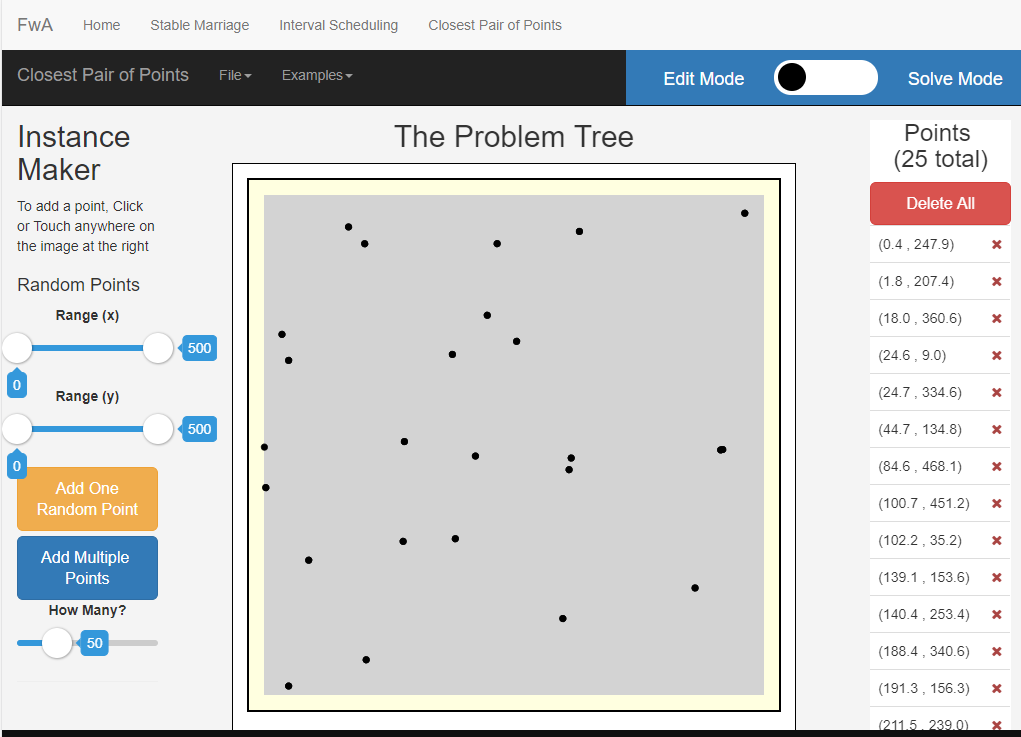
\includegraphics[width=\linewidth]
	{images/closest-pair-of-points/cpop-edit.png}
	\label{fig-cpop-edit}
	\centering
\end{figure}
\textit{Figure \ref{fig-cpop-edit}} shows the Closest Pair of Points
page upon first visiting it. 
In the center of the page is the \textsc{Display}: a square grid
with 25 random points in it. On the left is the \textsc{Instance Maker} 
and on the right is a table of coordinates for all the points in the grid.
\subsection{Instance Maker}
The \textsc{Instance Maker} consists of an interface to add points to the grid
and delete points from the grid. Too add a point, the simplest way is to 
click on the grid, and a point will be created at that location. 
An alternative method of adding points is by clicking one of the two available buttons.
These buttons add a random point to the grid. 
The number of points added by the ``Add Multiple Points'' 
button is determined by the slider below it.
\newline\newline
The user can specify the area where they want the random points to be in 
by changing the two sliders above the points. 
When these sliders are moved, the gray box inside the grid will change its size
and location to reflect the values in the sliders 
(see \textit{Figure \ref{fig-cpop-range}})
\newline\newline
\begin{figure}[H]
	\caption{Changing the Range for Random Points}
	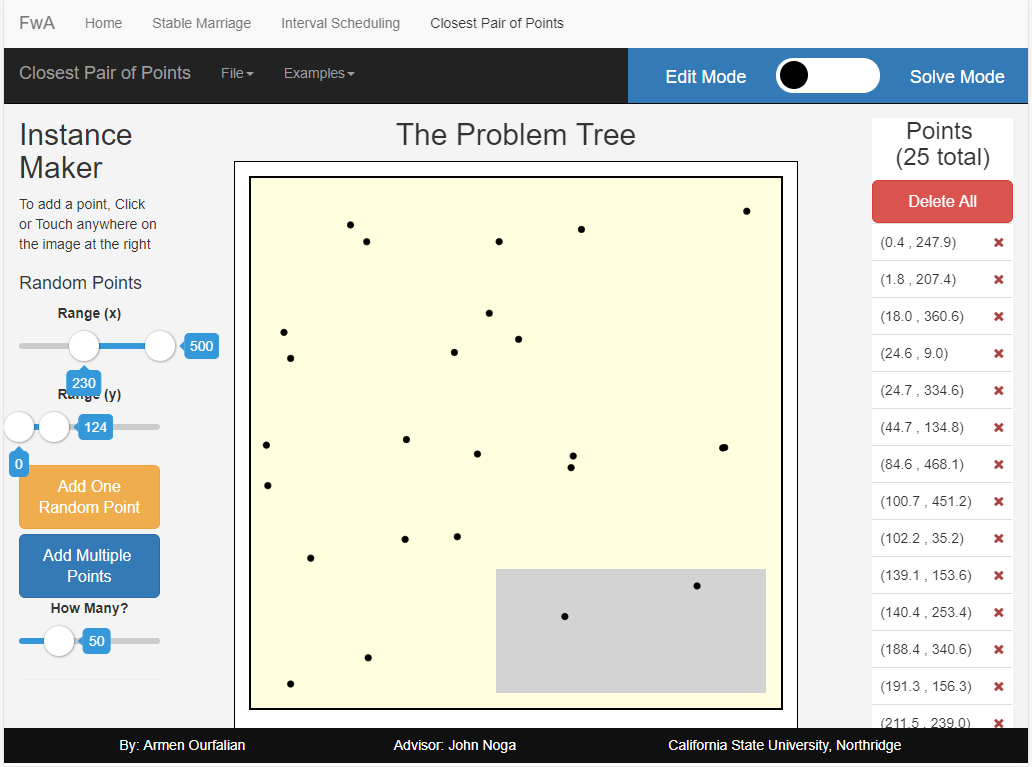
\includegraphics[width=\linewidth]
	{images/closest-pair-of-points/cpop-range.png}
	\label{fig-cpop-range}
	\centering
\end{figure}
\hspace{-0.3in}
To delete points, the user can click on the red X next to the coordinates
of the points they wan to delete. For the sake of clarity, when they 
move the mouse (or tap on) the coordinates, the point will change its 
color to red to identify itself. Alternatively, if the user wishes 
to delete all the points at once, they may do so by clicking the ``Delete All'' 
button above the list of coordinates. 
\subsection{Solver}
\begin{figure}[H]
	\caption{Closest Pair of Points in Solve Mode}
	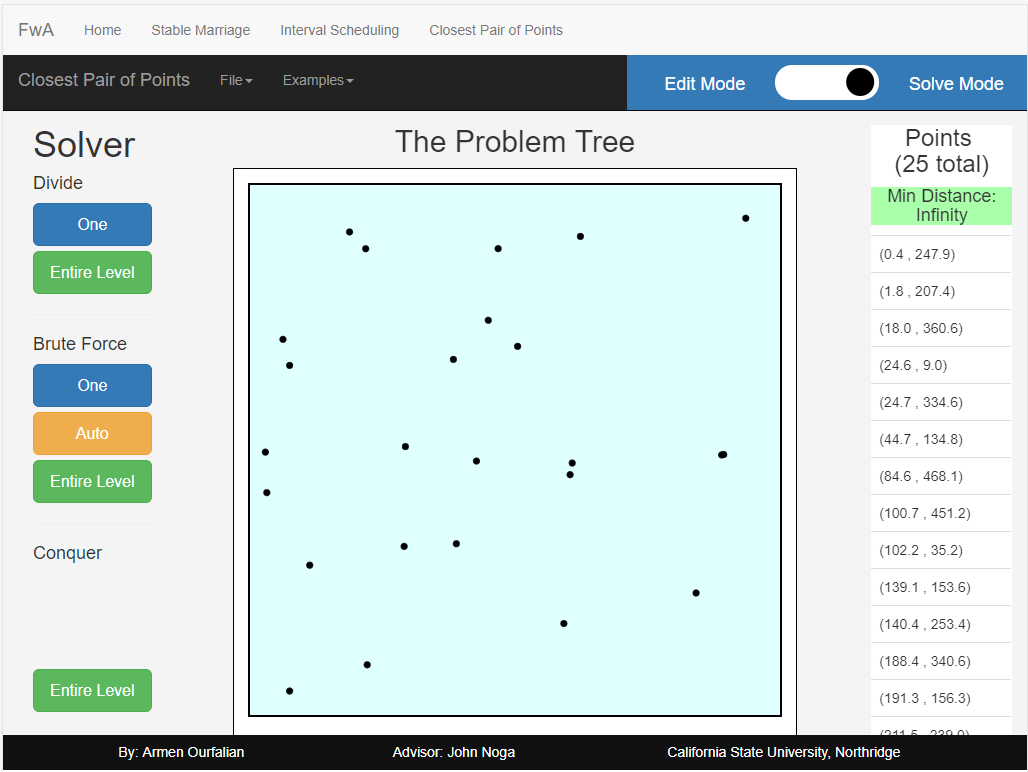
\includegraphics[width=\linewidth]
	{images/closest-pair-of-points/cpop-solver-1.png}
	\label{fig-cpop-solver-1}
	\centering
\end{figure}
\hspace{-0.3in}
\textit{Figure \ref{fig-cpop-solver-1}} shows the Closest Pair of Points page in 
Solve mode. The buttons and sliders to add or delete points have disappeared, 
and in their place are a new set of buttons on the left side. 
These buttons provide three functions: Divide, Brute Force, and Conquer.
Furthermore, each function comes in up to three varieties: 
\textbf{One} (blue), \textbf{Auto} (yellow), and \textbf{Entire Level} (green). 
Some of these buttons disappear if they are disabled, and reappear when they 
may be pressed. 
Also, the list of coordinates now also specifies what the current minimum distance
is for any two points on the grid. When Solve Mode is first entered, this 
distance is Infinity (because no distances have been checked yet).
\subsubsection{Divide}
\begin{figure}[H]
	\caption{Dividing a Grid}
	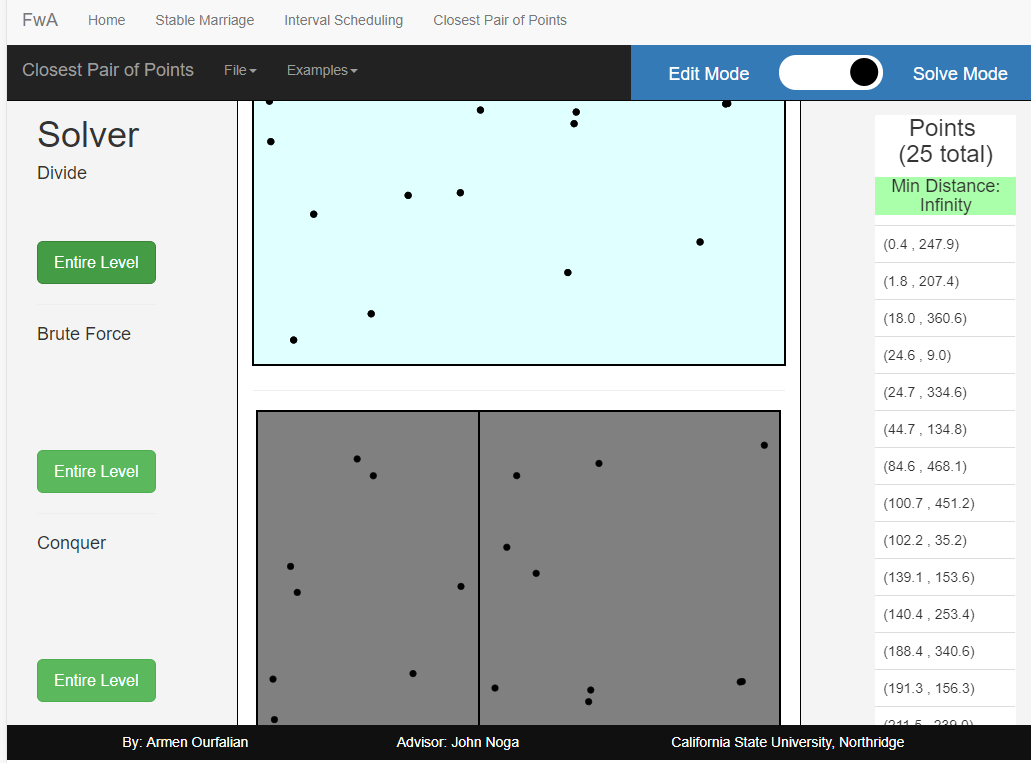
\includegraphics[width=\linewidth]
	{images/closest-pair-of-points/cpop-divide.png}
	\label{fig-cpop-divide}
	\centering
\end{figure}
\hspace{-0.3in}
\textit{Figure \ref{fig-cpop-divide}} shows what happens after either of the
``Divide'' buttons are clicked. 
The grid separates into two smaller grids. 
Each smaller grid has half the number of points as the original grid, either
the left half or the right half.
Now that there is more than one grid on the page, the user can select a grid
by clicking on it. The selected grid will be a light blue color whereas the 
other grids will be a dark gray. Clicking a button will only affect the 
selected grid, with the exception of the ``Entire Level'' buttons. 
``Divide Entire Level'' will perform the Divide function on 
every single grid that is at the same horizontal level as the selected grid. 
A grid can only be divided if it has more than three points. 
\subsubsection{Brute Force}
\begin{figure}[H]
	\caption{Brute Force}
	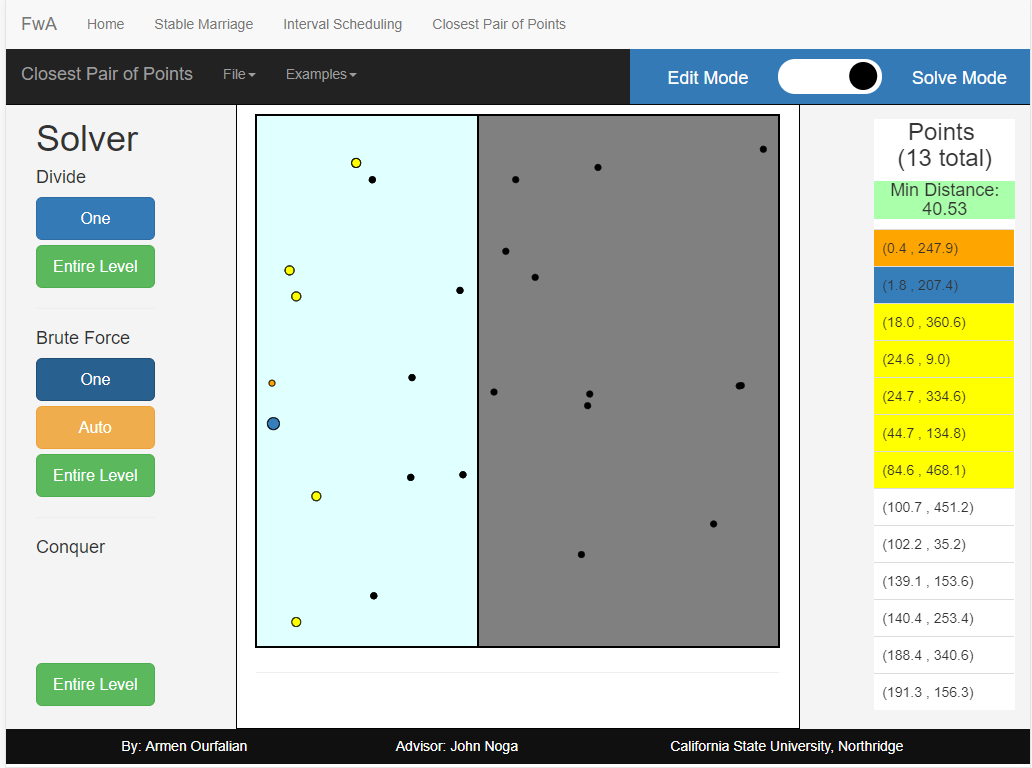
\includegraphics[width=\linewidth]
	{images/closest-pair-of-points/cpop-brute-force.png}
	\label{fig-cpop-brute-force}
	\centering
\end{figure}
\hspace{-0.3in}
When a grid has three or fewer points in it, the 
only function that a user can perform on it is Brute Force. 
To Brute Force a problem means to try every possible result and 
take the best one. In this case, the Brute Force function will check the distance
between every pair of points, and take the minimum of those.
\newline\newline
Clicking the ``Brute Force One'' button will turn one of the points in the grid blue
(the leftmost point). Each successive click will turn the next point in the list yellow, 
signifying the distance between that point and the blue point has been checked. 
When all points have been turned yellow, the blue point becomes orange, and the first 
yellow point becomes the new blue point (See \textit{Figure \ref{fig-cpop-brute-force}}. 
This button serves as an example of why 
brute forcing is not a good option for most problems; any time the number of points
is larger than $9$ or $10$, this process gets very tiresome, tedious, and boring. 
\newline\newline
The ``Auto'' option for Brute Force will perform the entire brute force operation in 
one click, and the ``Entire Level'' option will perform it on every grid at the same 
horizontal level as the selected grid. 
Although these two buttons go against good AV practices, their purpose is to 
speed up a process that could take up a lot of time. 
By using these buttons a lecturer can skip ahead to the more interesting parts 
of the discussion
\subsubsection{Conquer}
\hspace{-0.3in}
Conquering is the complement to Dividing. 
Two smaller grids that have both already been solved
are combined back into the original, larger grid. 
The new minimum distances is the smaller of their minimum distances. 
However, there is a strip in the middle of the two grids where 
the distance between the points has not been checked. 
The conquer function serves to check the points that are in this strip
to see if any two points are closer than the minimum distance. 
\newline\newline
The conquer function is similar to the Brute Force function in many ways: 
they both iterate through a set of points, 
changing the colors of points. 
However, the conquer function has a much smaller time complexity 
because each point is being checked with a finite number of other points. 
\newline\newline
\begin{figure}[H]
	\caption{Conquering a Grid}
	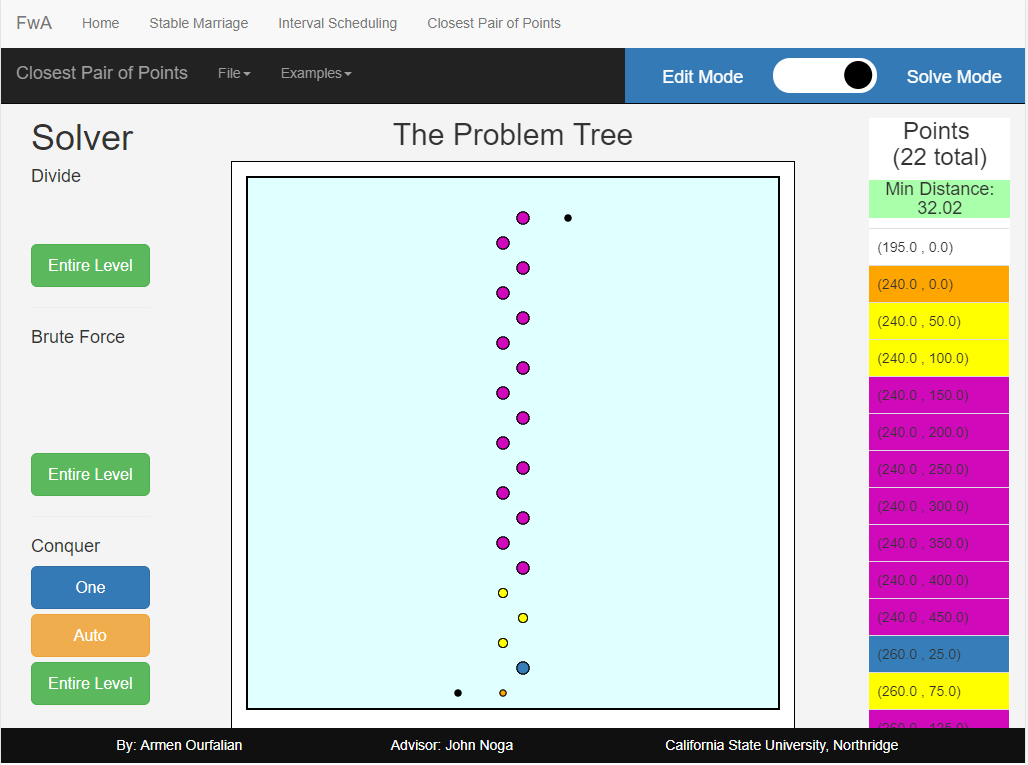
\includegraphics[width=\linewidth]
	{images/closest-pair-of-points/cpop-conquer.png}
	\label{fig-cpop-conquer}
	\centering
\end{figure}
\hspace{-0.3in}
Clicking on the ``Conquer One'' button will turn all of the points
inside of the strip to a purple color. Then, each successive click 
will behave exactly like the Brute Force function. 
The bottom-most point in the strip turns blue, and its distance is checked with 
the next 8 points (that are also in the strip). Afterwards, this point is 
turned orange, the next point is turned blue, and the process is repeated
(see \textit{Figure \ref{fig-cpop-conquer}}). 
\newline\newline
Since each point is being checked with only the next 8, this process is much 
less time-consuming than the brute force function. Yet it can still take a
very long time to complete. For that reason, the ``Conquer Auto'' button 
will automate this process and only show the results. Similarly, the 
``Conquer Entire Level'' button will perform the Conquer Auto function
on each grid at the same horizontal level as the selected grid. 
Note that a grid can only be conquered if it has been divided and if 
\underline{both} of its sub-grids have been fully solved 
(either through brute force or through conquering). 